\chapter{Alternate Loss Functions}

In chapter two we introduced the idea of a loss function.
We used the 0-1 loss function to make decision of which class to place an object in given its attributes.
In this chapter we will investigate some alternate loss functions that make better use of the structure of the insurance problem.

When classifying the insurance risk of a vehicle we return a class on an integer of scale of -2 to 3.
The 0-1 loss function assigns a loss of 1 to any risk rating that is not the true risk rating, regardless of how close it is.
We will test alternate choices for the loss function by measuring the accuracy and mean squared error.
We will use the expected posterior estimates with the uniform prior as described in the previous chapter.

Our selection of loss functions are based on those found in Lee \cite{Lee12}.

\section{The Loss Functions}
\subsection{0-1 Loss Function}
Previously we considered the 0-1 loss function.
To recap this is defined by:
\begin{equation}
	L(c, \hat{c}) = 
	\begin{cases}
		0 & \text{if}\ c = \hat{c} \\
		1 & \text{otherwise}
	\end{cases}
\end{equation}

The expected loss is:
\begin{equation}
	E(L) = \sum_{c \in \mathcal{C}} L(c, \hat{c})P(c \mid \mathbf{a}) = 1 - P(\hat{c} \mid \mathbf{a})
\end{equation}

So to minimize our expected loss we choose:
\begin{equation}\label{map}
	\hat c = \arg\max_{c \in \mathcal{C}} P(c)\prod_{i=1}^{k}P(a_i \mid c)
\end{equation}
This is known as the maximum a posteriori (MAP) estimate.

\subsection{Squared Differences}
The squared differences loss function is defined as:
\begin{equation}
	L(c, \hat{c}) = (c - \hat{c})^2
\end{equation}
This assigns greater loss to risk ratings that are further away from the true value.

For this function the expected loss is:
\begin{equation}
	E(L) = \sum_{c \in \mathcal{C}} (c - \hat{c})^2P(c \mid \mathbf{a}) 
\end{equation}

Differentiating this with respect to $\hat{c}$ gives:
\begin{equation}
	\frac{\partial}{\partial \hat{c}} E(L) = \sum_{c \in \mathcal{C}} (-2c + 2\hat{c})P(c \mid \mathbf{a}) 
\end{equation}
Setting this equal to zero gives:
\begin{align}
	\sum_{c \in \mathcal{C}} cP(c \mid \mathbf{a}) & = \sum_{c \in \mathcal{C}} \hat{c}P(c \mid \mathbf{a}) \\
	E(c \mid \mathbf{a}) & = \hat{c}
\end{align}
So the estimate which minimizes the loss function is the expected class.
In the context of our problem the estimated class must be an integer, however this expected value may not be.

\subsection{Absolute Difference}
Finally we have the absolute difference loss function:
\begin{equation}
	L(c, \hat{c}) = | c - \hat{c} |
\end{equation}
Once again this assigns greater loss to risk ratings that are further away from the true value.

For this function the expected loss is:
\begin{align}
	E(L) & = \sum_{c \in \mathcal{C}} |c - \hat{c}|P(c \mid \mathbf{a}) \\
	     & = \sum_{c < \hat{c}} (\hat{c} - c)P(c \mid \mathbf{a}) - \sum_{c \geq \hat{c}} (\hat{c} - c)P(c \mid \mathbf{a})
\end{align}

Differentiating this with respect to $\hat{c}$ gives:
\begin{align}
	\frac{\partial}{\partial \hat{c}} E(L) & = \sum_{c < \hat{c}} P(c \mid \mathbf{a}) - \sum_{c \geq \hat{c}} P(c \mid \mathbf{a}) \\
	& = \sum_{c \leq \hat{c}} P(c \mid \mathbf{a}) - \sum_{c \geq \hat{c}} P(c \mid \mathbf{a})
\end{align}
Setting this equal to zero gives:
\begin{align}
	\sum_{c \leq \hat{c}} P(c \mid \mathbf{a}) & = \sum_{c \geq \hat{c}} P(c \mid \mathbf{a}) \\
	P(c \leq \hat{c} \mid \mathbf{a}) & = P(c \geq \hat{c} \mid \mathbf{a})
\end{align}
So the estimate that minimizes expected loss for this loss function is the median value.
This may be difficult to define on our data set.
For example suppose class -3 had $P(C = -2 \mid \mathbf{a}) = 0.5 = P(C=3 \mid \mathbf{a})$ then any class could reasonably be considered the median and therefore minimize our expected loss.
When more than one risk rating could be reasonably considered the median we will choose one at random.

\section{Application}
We will now apply these loss functions to our automobile data set and measure accuracy and mean squared error.
We will also investigate how often the assigned classes agree.

As the expected posterior estimates perform better than the maximum likelihood estimates we shall use these to estimate the required probabilities.
We will also use the uniform hyper parameters and set $s=1$.

Using 10-fold cross validation our various loss functions perform as follow.

\begin{figure}
	\centering
	\begin{subfigure}{.5\textwidth}
		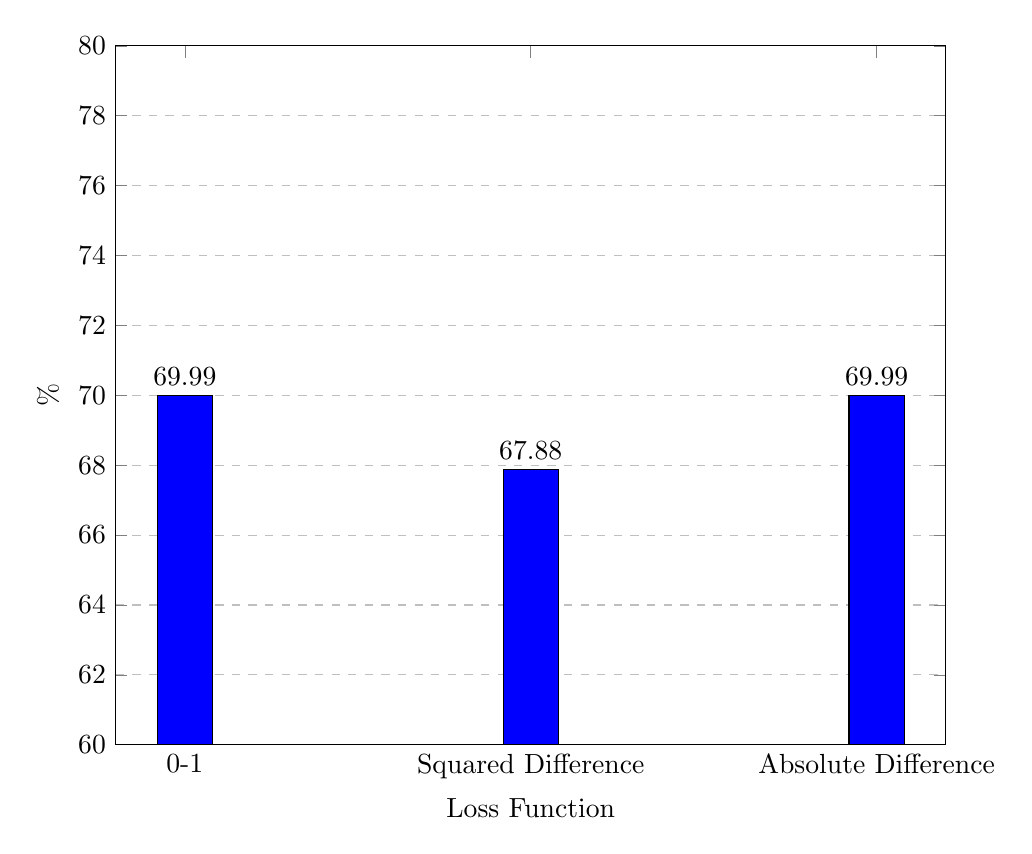
\begin{tikzpicture}
		\begin{axis}[
		    xlabel={Loss Function},
		    ylabel={\%},
		    width=\textwidth,
		    bar width=20pt,
		    symbolic x coords={0-1,Squared Difference,Absolute Difference},
		    ymin=60, ymax=80,
		    ymajorgrids=true,
		    grid style=dashed,
		    nodes near coords,
		    xtick=data]
		    \addplot[ybar,fill=blue] coordinates {
		        (0-1,69.99)
		        (Squared Difference,67.88)
		        (Absolute Difference,69.99)
		    };
		\end{axis}
		\end{tikzpicture}
		\caption{Accuracy}
	\end{subfigure}%
	\begin{subfigure}{.5\textwidth}
		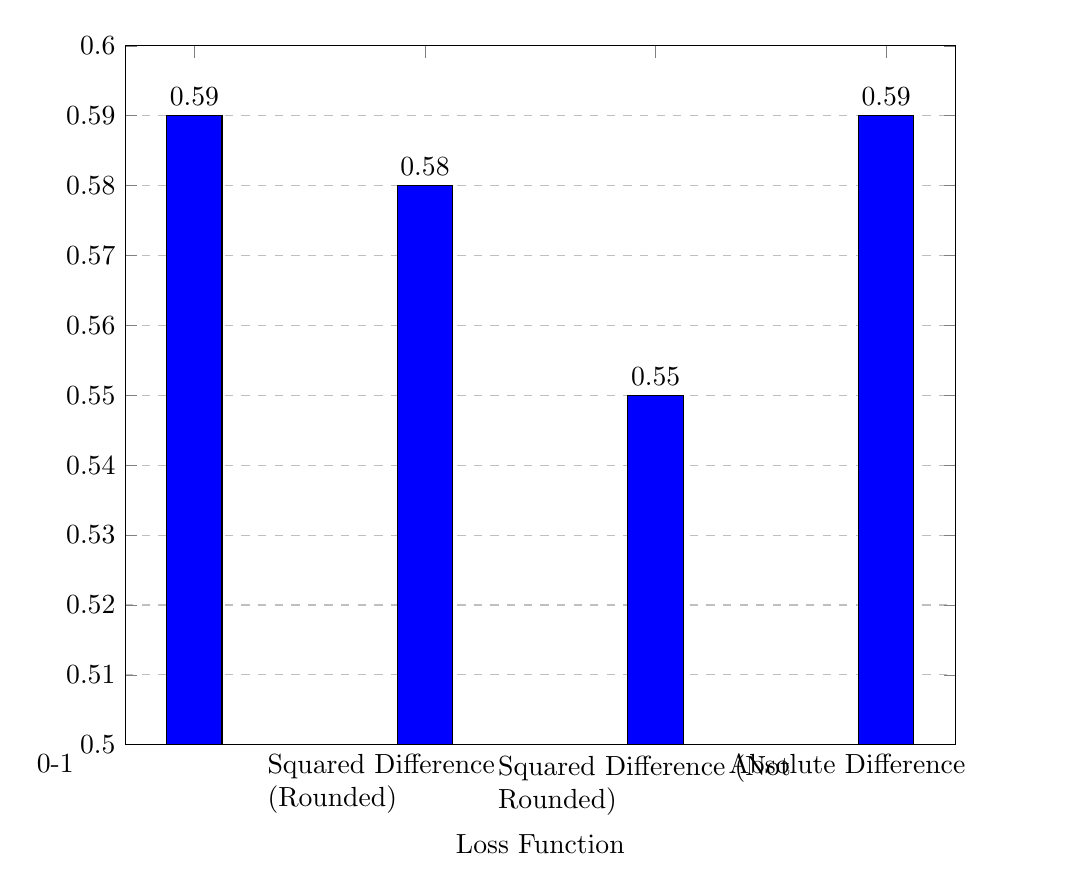
\begin{tikzpicture}
		\begin{axis}[
		    xlabel={Loss Function},
		    width=\textwidth,
		    bar width=20pt,
		    ymin=0.5, ymax=0.6,
		    ymajorgrids=true,
		    grid style=dashed,
		    nodes near coords,
		    symbolic x coords={0-1,Squared Difference (Rounded), Squared Difference (Not Rounded),Absolute Difference},
		    xtick=data,
		    x tick label style={text width=4cm}]
		    \addplot[ybar,fill=blue] coordinates {
		        (0-1,0.59)
		        (Squared Difference (Rounded),0.58)
		        (Squared Difference (Not Rounded), 0.55)
		        (Absolute Difference,0.59)
		    };
		\end{axis}
		\end{tikzpicture}
		\caption{MSE}
	\end{subfigure}
\end{figure}

Note that the 0-1 loss function and the absolute difference loss function perform the same.
The squared difference loss function performs slightly worse in the accuracy metric however scores better for MSE.

The 0-1 loss function and absolute differences loss function assign classes in a very similar manner.
This is due to there often being a $\hat{c} \in \mathcal{C}$ with a much greater $P(c \mid \mathbf{a})$.
When this is the case $\hat{c}$ is the choice for both the 0-1 loss function and the absolute difference loss functions.

The squared difference loss function differs from these two slightly as it is affected more by outliers.

\section{Further Loss Functions}
Here we have considered three common choices for the loss function however there are other options available.
We could even choose a loss function that is tailored to the problem at hand.
For example we could consider the loss function which assigns greater loss if we underestimate the risk rating of vehicle.